\documentclass[conference]{IEEEtran}
\usepackage{cite}
\usepackage{amsmath,amssymb}
\usepackage{graphicx}
\usepackage{textcomp}
\usepackage{xcolor}
\usepackage{booktabs}
\usepackage{multirow}
\usepackage{url}
\usepackage{hyperref}
\usepackage{balance}

\begin{document}

\title{From Passing Tests to Finding Failures: Teaching Exploratory and Robustness-Oriented Testing with Fuzzing}

\author{
\IEEEauthorblockN{
Author One\IEEEauthorrefmark{1}\IEEEauthorrefmark{2},
Author Two\IEEEauthorrefmark{1},
Author Three\IEEEauthorrefmark{1},
Author Four\IEEEauthorrefmark{1}\IEEEauthorrefmark{2}
}
\IEEEauthorblockA{\IEEEauthorrefmark{1}Affiliation One, City, Country}
\IEEEauthorblockA{\IEEEauthorrefmark{2}Affiliation Two, Institution, City, Country}
\{email1, email2, email3\}@domain.com, email4@domain.com
}

\maketitle

\begin{abstract}
Most software testing education focuses on confirming expected behavior, leaving students ill-equipped to discover unexpected failures.
This paper presents a structured classroom workshop that uses grammar-based fuzz testing with \emph{Fandango} to shift master's students toward exploratory and robustness-oriented testing thinking.
The workshop follows a four-phase pedagogical design: conceptual introduction, instructor live demonstration with a deliberately buggy program, guided student replication using shared materials, and an open-ended extension activity in which students introduce their own bugs or write new programs to fuzz.
We evaluated the workshop with 22 students, collecting pre/post self-assessment questionnaires ($N = 20$ matched pairs) and post-session perception data.
Results show large, statistically significant gains in domain-specific familiarity: grammar-based fuzzing knowledge increased by $+2.05$ points ($p < 0.001$, $r = 0.877$) and understanding of random-vs.-grammar fuzzing by $+2.10$ ($p < 0.001$, $r = 0.877$).
Students reported good usability (3.90/5) and engagement (3.87/5).
Open-ended responses also indicated an emergent connection between fuzzing and security-aware reasoning.
We discuss how grammar-based fuzzing can serve as an accessible, engaging entry point for exploratory testing mindsets in general software engineering courses.
\end{abstract}

\begin{IEEEkeywords}
Fuzz Testing, Software Testing Education, Exploratory Testing, Grammar-Based Fuzzing, Security-Aware Testing, Active Learning
\end{IEEEkeywords}

% ===========================================================================
\section{Introduction}
\label{sec:intro}
% ===========================================================================

A fundamental limitation of traditional software testing education is its emphasis on \emph{correctness validation}: students learn to write test cases that confirm expected outputs for expected inputs.
While necessary, this approach cultivates a mindset poorly suited for discovering the failures that matter most in practice---unexpected inputs, edge cases, malformed data, and adversarial conditions that no developer initially anticipated.

Consider a simple scenario: a developer writes a command-line calculator and verifies it works for \texttt{ADD 2 3} and \texttt{MUL 4 5}.
All tests pass.
But what happens when the input is \texttt{DIV 7 0}?
Or \texttt{ADD 999999 999999}?
Or simply an empty string?
Traditional testing rarely finds these failures because it tests what developers \emph{expect}, not what programs \emph{cannot handle}.

Fuzz testing---the automated generation of unexpected, malformed, or boundary inputs---directly addresses this gap~\cite{miller1990empirical}.
In particular, \emph{grammar-based fuzzing} generates structured inputs from formal grammar specifications, enabling systematic exploration of a program's input space in a way that is both principled and comprehensible to learners.
Unlike random fuzzing, grammar-based fuzzing produces syntactically meaningful inputs, making the connection between input structure and program behavior explicit and observable.

Despite its industrial prevalence~\cite{manes2019art}, fuzzing remains largely absent from software testing curricula.
Barriers include perceived complexity, lack of classroom-friendly tooling, and insufficient pedagogical frameworks connecting fuzzing to broader testing goals.

This paper presents a structured classroom workshop using \emph{Fandango}~\cite{fandango2025}, an open-source Python grammar-based fuzzer, to introduce exploratory and robustness-oriented testing thinking to master's students.
The workshop was designed not merely as a tool demonstration but as a \emph{mindset intervention}: helping students shift from asking ``does this program produce the right output?'' to asking ``what inputs could break this program?''

The study is guided by three research questions:
\begin{description}
    \item[RQ1] To what extent does the workshop improve students' familiarity with fuzz testing concepts and self-assessed confidence in exploratory testing?
    \item[RQ2] How do students perceive the workshop in terms of engagement, perceived learning, usability, and cognitive load?
    \item[RQ3] What difficulties do students encounter, and what do they reveal about the challenges of introducing fuzzing in educational contexts?
\end{description}

The contributions of this paper are threefold.
First, we present a structured, replicable pedagogical design for teaching grammar-based fuzzing that progresses from passive observation to active experimentation.
Second, we report empirical evidence of significant learning gains ($p < 0.001$, large effect sizes $r \geq 0.877$) for core fuzzing concepts.
Third, we identify the open-ended extension phase---where students break programs of their own design---as particularly effective for developing adversarial testing reasoning.

% ===========================================================================
\section{Background and Related Work}
\label{sec:background}
% ===========================================================================

\subsection{Exploratory and Robustness-Oriented Testing}

Traditional software testing education is grounded in correctness validation: given known inputs, verify that outputs match expected values~\cite{garousi2020testing}.
This approach produces competent test writers but may not develop the adversarial reasoning, edge-case awareness, and robustness thinking required in practice~\cite{ammann2016introduction}.
Students trained exclusively on example-based testing tend to underestimate the failure space, particularly for unexpected or malformed inputs~\cite{mccauley2008debugging}.

Exploratory testing~\cite{whittaker2009exploratory} frames testing as an investigative activity in which testers actively seek failures rather than confirm functionality.
Robustness testing extends this by explicitly targeting program behavior under abnormal or boundary conditions~\cite{manes2019art}.
Fuzzing operationalizes both---it explores the input space automatically and targets robustness by design.

\subsection{Fuzz Testing: Concepts and Educational Potential}

Fuzz testing was introduced by Miller et al.~\cite{miller1990empirical} and has become a standard industrial technique~\cite{klees2018evaluating}.
Modern fuzzers such as AFL~\cite{afl2021} and LibFuzzer operate at scale in industrial codebases.
Grammar-based fuzzing~\cite{aschermann2019nautilus, zeller2019fuzzing} generates structured inputs from formal specifications, producing human-readable test cases that illuminate the relationship between input format and program behavior.
This makes grammar-based fuzzing particularly suited for educational settings: students can read, modify, and reason about the generated inputs.

Despite its importance, fuzzing is rarely taught in software engineering courses and is typically framed as a security technique rather than a general testing strategy~\cite{klees2018evaluating}.
This framing limits its uptake in non-security courses, where robustness testing is equally valuable.

\subsection{Active Learning and Pedagogical Design}

The workshop design draws on experiential learning theory~\cite{kolb1984experiential}, which posits that effective learning occurs through cycles of concrete experience, reflective observation, and active experimentation.
The progression from instructor demonstration to guided replication to open-ended extension reflects a deliberate scaffolding strategy: students first observe, then reproduce, then independently apply.

Problem-based learning~\cite{hmelo2004problem} and inquiry-based approaches~\cite{prince2004active} further support this structure.
The extension phase---in which students design their own programs and attempt to break them with a fuzzer---is an authentic inquiry task with no predetermined answer.

% ===========================================================================
\section{Methodology}
\label{sec:methodology}
% ===========================================================================

\subsection{Participants and Context}

Participants were 22 master's students enrolled in a software engineering course at the Universidade da Beira Interior, Portugal.
Most (21/22) were from Computer Science or Software Engineering programs with intermediate programming experience.
Most reported little or no prior exposure to fuzz testing.
Participation in the research evaluation was voluntary, anonymous, and conducted under informed consent.

\subsection{Workshop Design}

The workshop lasted approximately 100~minutes and followed a four-phase pedagogical structure, illustrated in Fig.~\ref{fig:workflow}.

\begin{figure}[t]
\centering
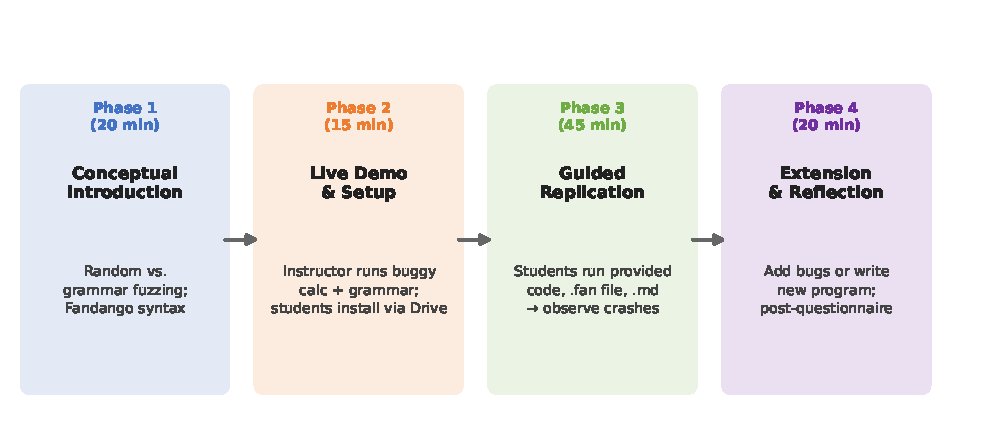
\includegraphics[width=\columnwidth]{figures/fig_fandango_workflow.pdf}
\caption{Workshop workflow: four progressive phases from conceptual introduction to open-ended extension.}
\label{fig:workflow}
\end{figure}

\subsubsection{Phase 1 --- Conceptual Introduction (20~min)}
The instructor presented the limitations of example-based testing using concrete examples, introduced the concept of fuzz testing, explained the difference between random and grammar-based fuzzing, and demonstrated the Fandango grammar syntax.

\subsubsection{Phase 2 --- Live Demonstration (15~min)}
The instructor ran a live fuzzing session using a deliberately buggy Python calculator program and a corresponding Fandango grammar file (\texttt{.fan}).
Students observed crashes in real time as the fuzzer generated inputs such as \texttt{DIV 7 0} and malformed expressions.
The instructor then analyzed a crash trace with the class, identifying the root cause and discussing how a defensive fix would look.

\subsubsection{Phase 3 --- Guided Replication (45~min)}
The instructor shared all materials with students via Google Drive: the buggy Python program, the Fandango grammar file (\texttt{.fan}), and a Markdown guide (\texttt{.md}) with step-by-step instructions for activating a Python virtual environment and running the fuzzer.
Students installed Fandango, ran the provided grammar against the target program, and observed the same crashes the instructor had demonstrated.
The instructor circulated to assist with installation and execution issues.
After successfully reproducing the fuzzing session, students were guided to modify the grammar to generate specific input classes (e.g., negative numbers, very large values, empty strings) and observe how each modification affected crash discovery.

\subsubsection{Phase 4 --- Open-Ended Extension (20~min)}
Students were given two options: (a)~introduce one or more deliberate bugs into the instructor's calculator program and attempt to verify whether the fuzzer could detect the new faults; or (b)~write a new Python program of their choice and repeat the entire fuzzing process from grammar design to crash analysis.
This phase encouraged students to reason adversarially: to think as both developer and tester simultaneously.
A short group reflection and post-session questionnaire concluded the workshop.

\subsection{Data Collection}

\subsubsection{Pre-Activity Questionnaire}
Background information; seven Likert self-assessment items (5-point scale) measuring: familiarity with fuzz testing, familiarity with grammar-based fuzzing, CLI confidence, edge-case understanding, automated test generation understanding, crash interpretation confidence, and understanding of the random-vs.-grammar distinction; one MCQ on grammar-based fuzzing definition.

\subsubsection{Post-Activity Questionnaire}
Same seven Likert items and MCQ; plus post-only constructs: perceived learning (5~items), engagement (3~items), usability (2~items), cognitive load (3~items), and four open-ended questions.

\subsubsection{Anonymous Matching}
Participants generated a personal code (last two digits of phone number + birth month + first letter of first name) used across both questionnaires.
Of 22 participants, 20 provided matched pre/post responses; one provided only a pre-session response.
All paired analysis uses $N = 20$.

\subsection{Data Analysis}

Pre/post Likert differences were tested using the Wilcoxon signed-rank test with effect size $r = |Z|/\sqrt{N}$.
Construct means were computed for post-session perception items.
Open-ended responses were analyzed using lightweight thematic coding.

% ===========================================================================
\section{Results}
\label{sec:results}
% ===========================================================================

\subsection{RQ1: Knowledge and Confidence Gains}

Table~\ref{tab:likert} reports pre/post self-assessment for all seven Likert items ($N = 20$).
Fig.~\ref{fig:prepost} visualizes the shifts across all items.

\begin{table}[htbp]
\caption{Pre/Post Self-Assessment ($N = 20$)}
\label{tab:likert}
\centering
\small
\begin{tabular}{lccccc}
\toprule
Item & Pre & Post & $\Delta$ & $p$ & $r$ \\
\midrule
Fuzz familiarity         & 1.80 & 3.55 & +1.75 & .000 & .855 \\
Grammar-fuzz famil.      & 1.60 & 3.65 & +2.05 & .000 & .877 \\
CLI confidence           & 2.90 & 3.50 & +0.60 & .017 & .567 \\
Edge-case underst.       & 3.60 & 3.85 & +0.25 & .322 & .285 \\
Auto-test generation     & 3.70 & 4.10 & +0.40 & .091 & .422 \\
Crash interpretation     & 3.00 & 3.45 & +0.45 & .033 & .513 \\
Random vs.\ grammar      & 1.65 & 3.75 & +2.10 & .000 & .877 \\
\bottomrule
\end{tabular}
\end{table}

\begin{figure}[htbp]
\centering
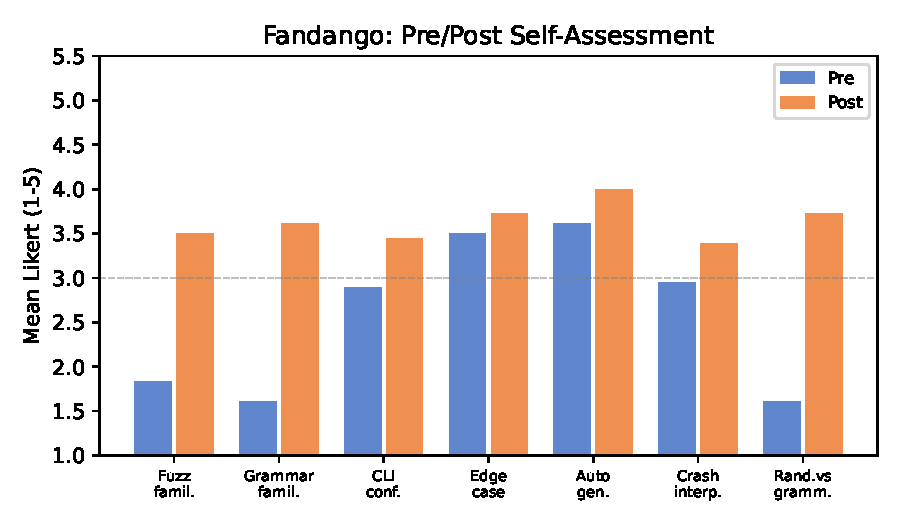
\includegraphics[width=\columnwidth]{figures/fig_fandango_prepost.pdf}
\caption{Pre/post self-assessment across seven Likert items. Largest gains on items directly addressed by the workshop.}
\label{fig:prepost}
\end{figure}

The largest gains were on the three items most directly addressed by the workshop.
Grammar-based fuzzing familiarity increased by $+2.05$ points ($p < 0.001$, $r = 0.877$, large effect), and understanding of the random-vs.-grammar distinction by $+2.10$ ($p < 0.001$, $r = 0.877$).
These gains reflect a very low pre-session baseline (mean $\approx$ 1.6/5), where large gains were possible precisely because students had almost no prior exposure to fuzzing.

CLI confidence showed a moderate, significant gain ($+0.60$, $p = 0.017$, $r = 0.567$), and crash interpretation improved significantly ($+0.45$, $p = 0.033$, $r = 0.513$).
Edge-case understanding and automated test generation showed positive but non-significant trends ($p > 0.05$), consistent with these being broader skills that a single session cannot fully develop.

\subsection{RQ2: Student Perception}

Table~\ref{tab:perception} summarizes post-session perception ($N = 20$), with Fig.~\ref{fig:perception} providing a visual overview.

\begin{table}[htbp]
\caption{Post-Session Perception ($N = 20$)}
\label{tab:perception}
\centering
\small
\begin{tabular}{lcc}
\toprule
Construct (items) & Mean & \% Agree \\
\midrule
Perceived Learning (5) & 3.73 & 60\% \\
Engagement (3)         & 3.87 & 62\% \\
Usability (2)          & 3.90 & 68\% \\
Cognitive Load (3)     & 3.32 & --- \\
\bottomrule
\end{tabular}
\end{table}

\begin{figure}[htbp]
\centering
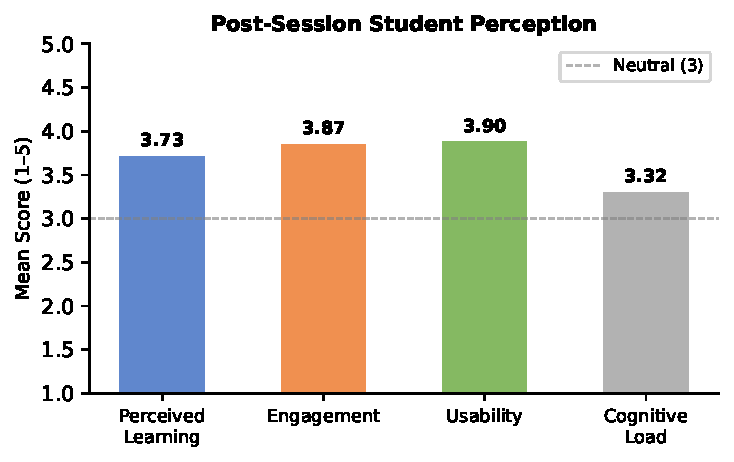
\includegraphics[width=\columnwidth]{figures/fig_fandango_perception.pdf}
\caption{Post-session perception: mean scores across four constructs. Dashed line indicates neutral (3).}
\label{fig:perception}
\end{figure}

Usability was rated highest (3.90/5), suggesting that Fandango's interface was accessible once installation was complete.
Engagement was good (3.87/5, 62\% agree).
Perceived learning was moderate (3.73/5, 60\% agree), which may reflect the conceptual novelty of the domain rather than dissatisfaction.
Cognitive load was moderate (3.32/5), consistent with the inherent complexity of fuzzing combined with CLI tool operation.

\subsection{RQ3: Student Difficulties and Qualitative Themes}

Thematic analysis of open-ended responses revealed four recurring themes:

\begin{enumerate}
    \item \textbf{Installation and environment friction:} The most frequently reported difficulty was tool setup, particularly on Windows (\emph{``problems installing Fandango,''} \emph{``version of Python,''} \emph{``pre requirements to make the activity run''}).
    \item \textbf{Conceptual novelty:} Students found the grammar specification syntax unfamiliar at first (\emph{``grammar-based fuzzing was hard to grasp initially''}).
    \item \textbf{Security awareness:} Multiple students connected crashes to potential vulnerabilities (\emph{``Analysing software crashes,''} \emph{``Crash demonstration''}).
    \item \textbf{Engagement with the extension phase:} Students valued hands-on experimentation (\emph{``I wanted to explore more grammars,''} \emph{``Tutorial instructions with a quick create bug, generate results, find bug, fix bug and repeat,''} \emph{``More practical in more hours''}).
\end{enumerate}

% ===========================================================================
\section{Discussion}
\label{sec:discussion}
% ===========================================================================

\subsection{The Pedagogical Progression: Observe, Reproduce, Break}

The three-stage activity structure---live demonstration, guided replication, open-ended extension---proved effective at scaffolding the transition from passive observation to active adversarial reasoning.

The live demonstration (Phase 2) provided the motivating experience: students saw a seemingly correct program produce unexpected crashes from simple, automatically generated inputs.
This concrete observation---not a lecture---is what makes fuzzing memorable as a testing technique.

The guided replication (Phase 3) ensured that all students could reproduce the experience independently, reinforcing the conceptual explanation with hands-on practice.
The provision of structured materials (Python program, grammar file, and step-by-step Markdown guide) via Google Drive removed the design barrier and allowed students to focus on the testing concepts rather than the tool mechanics.

The open-ended extension (Phase 4) was designed to encourage students to reason adversarially as both developer and tester simultaneously.
Open-ended responses suggest that students perceived this phase as particularly valuable, although no systematic log data were collected to quantify how many students completed it or what types of faults were discovered.
The dual perspective embedded in this phase---understanding not just that programs can fail, but \emph{why} they fail and \emph{how} to design inputs that expose specific failure modes---represents the core of the exploratory testing mindset this workshop aims to cultivate.

\subsection{Fuzzing as a Security Awareness Gateway}

An emergent qualitative theme in open-ended responses was the spontaneous connection students drew between observed crashes and potential vulnerabilities.
The workshop was not framed as a security course, yet several students---without prompting---linked unexpected program failures to security risks.
This suggests that fuzz testing activities may naturally support security-aware reasoning as a by-product, although this observation is based on qualitative responses and warrants further investigation before stronger claims can be made.

\subsection{Installation Friction: Barrier and Authentic Experience}

The dominant practical challenge---tool installation and environment configuration---warrants careful consideration.
On one hand, it consumed valuable activity time and caused frustration.
On the other hand, dependency management, platform-specific build requirements, and virtual environment configuration are authentic features of professional software engineering practice.
Exposing students to this friction---with instructor support to overcome it---contributes to professional readiness in ways that pre-configured cloud environments cannot replicate.

We recommend a hybrid approach: provide a pre-configured environment as a backup for students who cannot complete installation, while still guiding the installation process as part of the workshop.
This preserves the authentic experience for those who can complete it while ensuring no student is entirely excluded.

\subsection{Limitations of a Single Session}

Non-significant results for edge-case understanding ($p = 0.322$) and automated test generation ($p = 0.091$) indicate that broader exploratory testing competencies require more than a single workshop.
A single session can introduce vocabulary, motivate the mindset, and demonstrate the technique; sustained curriculum integration is necessary for deeper skill development.
Future workshops should build on this foundation with more complex grammars, multi-session activities, and integration with complementary techniques such as property-based testing and mutation testing.

% ===========================================================================
\section{Threats to Validity}
\label{sec:threats}
% ===========================================================================

\textbf{Internal validity.}
The pre/post design without a control group limits causal interpretation.
MCQ item reuse may introduce a testing effect.

\textbf{Construct validity.}
Self-reported Likert assessments may not capture actual skill acquisition.
The seven Likert items were designed for this study and have not been validated in prior work.

\textbf{External validity.}
Single cohort ($N = 22$) at one institution limits generalizability.
Results may differ with students of different backgrounds, different target programs, or different Fandango versions.

\textbf{Reliability.}
Cronbach's $\alpha$ for perceived learning ($0.879$), engagement ($0.858$), and usability ($0.812$) indicate acceptable to good internal consistency.
Cognitive load items showed lower consistency due to mixed item valence and are interpreted descriptively.

% ===========================================================================
\section{Conclusion}
\label{sec:conclusion}
% ===========================================================================

This paper presented a structured classroom workshop for teaching grammar-based fuzz testing as a vehicle for exploratory and robustness-oriented testing thinking.
The workshop's four-phase progression---conceptual introduction, live demonstration, guided replication, and open-ended extension---scaffolds students from passive observation to active adversarial reasoning.

Empirical results support significant learning gains: grammar-based fuzzing familiarity increased by $+2.05$ ($p < 0.001$, $r = 0.877$) and the random-vs.-grammar distinction by $+2.10$ ($p < 0.001$, $r = 0.877$).
Students rated the activity as engaging and usable, and open-ended responses suggested that the extension phase was particularly valued.
An emergent qualitative theme was the spontaneous connection students drew between observed crashes and potential security vulnerabilities, a finding that warrants further investigation.

Future work should investigate multi-session curricula that build on this foundation, longitudinal retention of the exploratory testing mindset, and the integration of grammar-based fuzzing with mutation testing and property-based testing.

\section*{Data Availability}
The replication package---including questionnaire data, analysis scripts, and workshop materials---is publicly available at: \url{https://github.com/aazaadef/Fandango-Workshop}

\section*{Acknowledgment}
This work was supported by FCT -- Funda\c{c}\~{a}o para a Ci\^{e}ncia e Tecnologia, I.P.\ by project reference UIDB/50008/2020 (DOI: \url{https://doi.org/10.54499/UIDB/50008/2020}) and by the doctoral grant PRT/BD/155023/2023.
The authors would also like to acknowledge the Promptme4Better project, funded by the European Union Erasmus+ Program and the Portugal National Agency under grant agreement number 2025-1-PT01-KA220-HED-000363565, and all partners involved in the project.
The authors used generative AI tools solely to support English language polishing and readability improvements.
All technical content, interpretations, and conclusions were created and verified by the authors, who take full responsibility for the final manuscript.

\balance
\bibliographystyle{IEEEtran}
\begin{thebibliography}{99}
\bibitem{fandango2025} ``Fandango: Grammar-Based Fuzzing Tool,'' 2025. Available: https://github.com/fandango-fuzzer/fandango
\bibitem{miller1990empirical} B.~P.~Miller, L.~Fredriksen, and B.~So, ``An Empirical Study of the Reliability of UNIX Utilities,'' \emph{Commun.\ ACM}, vol.~33, no.~12, pp.~32--44, 1990.
\bibitem{manes2019art} V.~J.~M.~Man\`{e}s et~al., ``The Art, Science, and Engineering of Fuzzing: A Survey,'' \emph{IEEE Trans.\ Softw.\ Eng.}, vol.~47, no.~11, pp.~2312--2331, 2021.
\bibitem{klees2018evaluating} G.~Klees et~al., ``Evaluating Fuzz Testing,'' in \emph{Proc.\ CCS '18}, ACM, 2018, pp.~2123--2138.
\bibitem{aschermann2019nautilus} C.~Aschermann et~al., ``NAUTILUS: Fishing for Deep Bugs with Grammars,'' in \emph{Proc.\ NDSS '19}, 2019.
\bibitem{zeller2019fuzzing} A.~Zeller, R.~Gopinath, M.~B\"{o}hme, G.~Fraser, and C.~Holler, ``The Fuzzing Book,'' 2019. Available: https://www.fuzzingbook.org/
\bibitem{afl2021} M.~Zalewski, ``American Fuzzy Lop (AFL),'' 2021. Available: https://lcamtuf.coredump.cx/afl/
\bibitem{whittaker2009exploratory} J.~A.~Whittaker, \emph{Exploratory Software Testing}. Addison-Wesley, 2009.
\bibitem{ammann2016introduction} P.~Ammann and J.~Offutt, \emph{Introduction to Software Testing}, 2nd~ed. Cambridge University Press, 2016.
\bibitem{garousi2020testing} V.~Garousi, A.~Rainer, P.~Lauv\aa{}s~Jr., and A.~Arcuri, ``Software-testing education: A systematic literature mapping,'' \emph{J.\ Syst.\ Softw.}, vol.~165, 2020.
\bibitem{mccauley2008debugging} R.~McCauley et~al., ``Debugging: a review of the literature from an educational perspective,'' \emph{Comput.\ Sci.\ Educ.}, vol.~18, no.~2, pp.~67--92, 2008.
\bibitem{kolb1984experiential} D.~A.~Kolb, \emph{Experiential Learning: Experience as the Source of Learning and Development}. Prentice-Hall, 1984.
\bibitem{hmelo2004problem} C.~E.~Hmelo-Silver, ``Problem-Based Learning: What and How Do Students Learn?'' \emph{Educ.\ Psychol.\ Rev.}, vol.~16, no.~3, pp.~235--266, 2004.
\bibitem{prince2004active} M.~Prince, ``Does Active Learning Work? A Review of the Research,'' \emph{J.\ Eng.\ Educ.}, vol.~93, no.~3, pp.~223--231, 2004.
\end{thebibliography}

\end{document}
